\documentclass[onecolumn,draftclsnofoot, 10pt, compsoc]{IEEEtran}

\usepackage{graphicx}
\usepackage[section]{placeins}
\usepackage{caption}

\usepackage{amssymb}                                         
\usepackage{amsmath}                                         
\usepackage{amsthm}                                

\usepackage{alltt}                                           
\usepackage{float}
\usepackage{color}
\usepackage{url}

\usepackage{balance}
\usepackage[TABBOTCAP, tight]{subfigure}
\usepackage{enumitem}
\usepackage{pstricks, pst-node}
\usepackage{url}
\usepackage{setspace}

\usepackage{etoolbox}
\AtBeginEnvironment{quote}{\singlespacing\vspace{-\topsep}\small}

%\input{pygments.tex}

\usepackage{geometry}
\geometry{left=0.75in,right=0.75in,top=0.75in,bottom=0.75in}
\parindent = 0.0 in
\parskip = 0.1 in

\usepackage{listings}
\lstset{language=C,caption={Descriptive Caption Text},label=DescriptiveLabel}
\lstdefinestyle{customc}{
	belowcaptionskip=1\baselineskip,
	breaklines=true,
	frame=L,
	xleftmargin=\parindent,
	language=C,
	showstringspaces=false,
	basicstyle=\footnotesize\ttfamily,
	keywordstyle=\bfseries\color{green!40!black},
	commentstyle=\itshape\color{purple!40!black},
	identifierstyle=\color{blue},
	stringstyle=\color{orange},
}

\lstdefinestyle{customasm}{
	belowcaptionskip=1\baselineskip,
	frame=L,
	xleftmargin=\parindent,
	language=[x86masm]Assembler,
	basicstyle=\footnotesize\ttfamily,
	commentstyle=\itshape\color{purple!40!black},
}


\def \ParSpace{\vspace{.75em}}
\def \GroupNumber{		17}
\def \Jeremy{			Jeremy Fischer}
\def \Class{		Operating Systems ii}
\def \School{	Oregon State University}
\def \Professor{		 Kevin McGrath}

\newcommand{\cred}[1]{{\color{red}#1}}
\newcommand{\cblue}[1]{{\color{blue}#1}}

\newcommand{\NameSigPair}[1]{
		\par
		\makebox[2.75in][r]{#1} \hfil 	\makebox[3.25in]{\makebox[2.25in]{\hrulefill} \hfill			
		\makebox[.75in]{\hrulefill}}
		\par\vspace{-12pt} \textit{
			\tiny\noindent
			\makebox[2.75in]{} \hfil		
			\makebox[3.25in]{
				\makebox[2.25in][r]{Signature} \hfill	\makebox[.75in][r]{Date}
			}
		}
}










%%%%%%%%%%%%%%%%%%%%%%%%%%%%%%%%%%%%%%%
\begin{document}
\begin{titlepage}
    \pagenumbering{gobble}
    \begin{singlespace}
    
\includegraphics[height=4cm]{coe.eps}
        \hfill  
        \par\vspace{.2in}
        \centering
        \scshape{
            \vspace{.5in}
            \textbf{\Huge\Class}\par
            \large{
            	\today \\Fall Term
        	}
            \vfill
            {\large Prepared for}\par
            \huge \School\par
            \vspace{5pt}
            {\Large{\Professor}\par}
            {\large Prepared by }\par
           % Group\GroupNumber\par
            \vspace{5pt}
            {\Large
                {\Jeremy}\par
            }
            \vspace{20pt}
        }
        \begin{abstract}
        	This document explores processes and threads, devices, memory management, and file systems in the Linux, FreeBSD, and Windows operating systems. 
        	Each section concludes with a comparison of the three's implementation.
        \end{abstract}     
    \end{singlespace}
\end{titlepage}
\newpage
\pagenumbering{arabic}
\tableofcontents
% 7. uncomment this (if applicable). Consider adding a page break.
%\listoffigures
%\listoftables
\clearpage


\section{Introduction}
	This document explores how the Linux, FreeBSD, and Windows operating systems approach processes and threads, devices, memory management, and file systems.
	The processes and threads section takes a look at what is considered a process and what is considered a thread, as well as CPU scheduling.
	Followed is the devices section, which analyzes the devices each operating system offers, the development resources, and I/O scheduling.
	The memory management section comes next, and is responsible for examining how each operating system handles memory, specifically virtual memory.
	The last section is about file systems, in which two popular file systems from each operating system are explored.

%************************PROCESSES AND THREADS************************%

\section{Processes and Threads}
	\subsection{Linux Implementation}
		\subsubsection{Processes}
			Each process has its own private resources, data, and associated statistics about itself so the OS can make good scheduling decisions. 
			In memory the process is divided into segments: Stack, Heap, and Text. Program code is converted into machine readable instructions and is stored in the Text segment. 
			Local function-variables that are automatically allocated go in the Stack. 
			And memory dynamically allocated by the program go in the Heap. 
			As memory is used by a process the stack and heap grow toward each other. 
			If a process has shared libraries then it is mapped into process memory which is placed between the stack and the heap.
			A process can either be independent or cooperating \cite{processesLinux}.
			\begin{itemize}
				\item An independent process cannot affect or be affected by the execution of another process
				\item Cooperating processes can affect or be affected by another process. This is usually done for information sharing
			\end{itemize}
	
			\ParSpace
			Each process has information associated to itself so the operating system can achieve certain tasks efficiently.  The operating system tracks\dots
			\begin{itemize}
				\item The memory the process is using as well as where in the memory the process is currently executing (instruction pointer)
				\item Any open files or network connections the process is using
				\item The amount of CPU time a process has used as well as the amount of RAM being consumed by the process
				\item Each process has a process ID so the OS can distinguish it from other processes. 
				\item The current process's parent i.e. the process that created the current process. This is done so the OS can handle permissions to resources efficiently
			\end{itemize}

			\ParSpace
			All processes are created from a parent process, except for the \textbf{init} process with is created by the OS kernel. 
			All other processes are a child of \textbf{init}  (parent of all parents).
			The \textbf{init}  process must remain alive for the entire time the system is up and running.
			The \textbf{init} process has a process ID of 1. 
			A process is created by its parent making a copy of itself - called forking.
			The child's memory space is initially an exact copy of its parent.
			The parent however, decides which resources to share with its child. Resources such as open file descriptors and open network connections are shared by default. The parent may decided not to share any resources, making the forked process independent.
			Once a child is initialized it is its own process that can run in parallel with the parent. 
			The parent can either wait on the child to finish doing its work before continuing, or it can continue on its own duties, or it can kill the child process.
			A child process can load a completely different program into its allocated memory, which replaces the copy of the parents program. This is called "exec-ing" due to it being done through the \textit{exec} command. 
	
		\subsubsection{Threads}
			A thread can be thought of as a light weight process. 
			As in, there's no need to allocate memory for the thread. 
			The thread instead shares the memory of the process that it is in (except the stack segment).
			Linux threads follow a co-operative multitasking scheme where the threads are executed sequentially. 
			However, the time to switch from one thread to the next is so incredibly fast that it appears they're running in parallel. 
			The downside to this scheme is that if one thread gets blocked then the whole process gets blocked \cite{threadsVidLinux}.
			Each thread is dependent on the process and other threads. They all share the same data. A thread can only access data within its process.
			Processes are the entities that group resources together. Threads are the entities that are actually scheduled for execution by the CPU.
			There are user threads and kernel threads \cite{threadsArtiLinux}:
			\begin{itemize}
				\item User threads are created and killed in user space. 
				The kernel is not aware of these threads, meaning it is not involved in their processing.
				\item Kernel threads are created and killed by the kernel. 
				Each thread that exists in the user space has a counterpart kernel thread. 
				Since these threads are managed by the kernel they follow preemptive multitasking - meaning the scheduler can stop a thread's execution so a higher priority thread can run. 
				In contrast to user threads, if a kernel thread gets blocked it doesn't cause the whole system to block since it follows a preemptive scheduling model. 
				However, switching from one thread to the next is slower for kernel threads.
			\end{itemize}
	
		\subsubsection{CPU Scheduling}
			The Completely Fair Scheduler, CFS, is a task scheduler that Linux introduced in version 2.6.23 \cite{schedulerLinux}. 
			Its goal is to utilize the CPU as efficiently as possible by handling resource allocation. 
			The scheduler uses red-black trees instead of run queues like Windows.
			The main idea is to have the tree remain balanced, providing a fair amount of processing time to each process relative to the others. 
			When a process isn't given a fair amount then they are given extra time to execute.
			The CFS maintains the amount of time provided to a given task in the virtual runtime. 
			The smaller a task's virtual runtime, i.e. the smaller amount of assigned processor time, the higher its priority. 
			The CFS also includes the concept of sleeper fairness to ensure that tasks that are not currently runnable (waiting for I/O, etc.) receive a fair share of the processor when they eventually need it \cite{schedulerLinux}.


	\subsection{Windows Implementation}
		\subsubsection{Processes}
			\begin{figure}[H]
				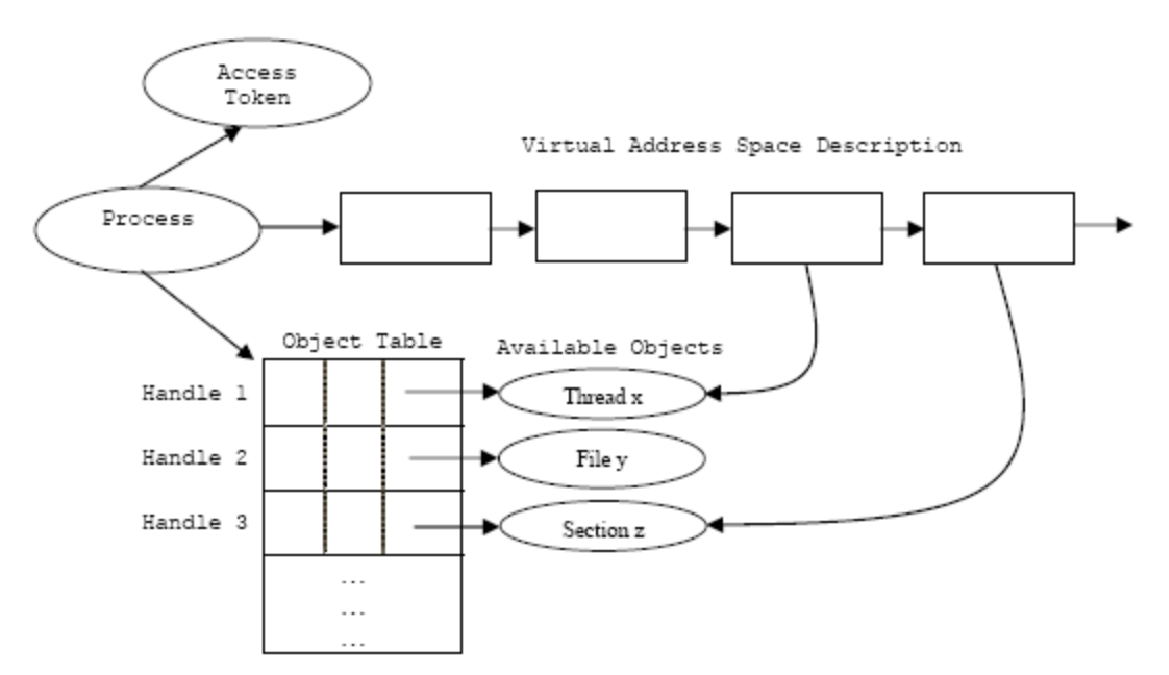
\includegraphics[width=.6\textwidth]{windowsProcessTemplate.eps}
				\centering
				\caption{Windows process object template used when creating a new process object \cite{windowsProcessMSDN}}
				\label{fig:mesh1}
			\end{figure}
		
			A Windows process has a virtual address space, executable code, open handles to system objects, a security context, a unique process identifier, environment variables, a priority class, minimum and maximum working set sizes, and at least one thread of execution \cite{windowsProcessMSDN}.
			Each process is represented as an object.
			When Windows creates a new process it uses the template outlined in figure \ref{fig:mesh1} to generate a new object instance. 
			The access token attached to each process lets the operating system know what the process has access to.
			When a process object is first created it is given an initial thread.
			This thread is refereed to as the \textit{primary thread}.
			Although a process starts with only one thread, each thread is capable of creating new ones.
	
		\subsubsection{Threads}
			A thread is the entity within a process that can be scheduled for execution. 
			All threads of a process share the virtual address space and system resources pertaining to its encompassing process. In addition, each thread maintains exception handlers, a scheduling priority, thread local storage, a unique thread identifier, and a set of structures the system will use to save the thread context until it is scheduled. The thread context includes the thread's set of machine registers, the kernel stack, a thread environment block, and a user stack in the address space of the thread's process. \cite{windowsProcessMSDN}.
			Threads are ranked in a priority based system. 
			There are 33 priority levels - zero is the lowest and 32 is the highest. 
			However, only the zero-page thread can obtain a priority level of zero (The zero-page thread is a system thread responsible for zeroing any free pages when there are no other threads that need to run.).
			The threads are prioritized by two general rules:
			\begin{itemize}
				\item The priority class of its process
				\item The priority level of the thread within the priority class of its process
			\end{itemize}
	
	
		\subsubsection{CPU Scheduling}
			The system treats all threads with the same priority as equal - i.e. there is no further favoring of threads then their priority level.
			All high priority threads are assigned a time-slice in a round-robin fashion. 
			In cases where no high priority threads are able to run (they're waiting), then time-slices are assigned to the next highest priority level of threads in the same round-robin fashion.
			When a higher priority thread stops waiting and is able to run, the system abruptly halts the lower priority threads, and assigns a full time-slice to the awakened higher priority thread.
			Windows maintains a queue of readily executable threads for each priority level \cite{windowsCSwitchesMSDN}.
			When a processor becomes available the following steps are taken by the system to allow the next thread to run:
			\begin{enumerate}
				\item Save the context of the thread that just finished executing.
				\item Place the thread that just finished executing at the end of the queue for its priority.
				\item Find the highest priority queue that contains ready threads.
				\item Remove the thread at the head of the queue, load its context, and execute it.
			\end{enumerate}
			This scheduling design prioritizes short jobs and I/O bound processes. 
			Another important note is that all processes get their priority boosted after a wait event. However, processes waiting for user I/O get a larger priority boost than processes waiting on disk I/O \cite{schedulerWindows}. 




	\subsection{FreeBSD Implementation}
		\subsubsection{Processes}
			\begin{figure}[H]
				\includegraphics[width=.55\textwidth]{FreeBSDProcess.eps}
				\centering
				\caption{FreeBSD process structure \cite{freeBSDProcess}}
				\label{fig:mesh2}
			\end{figure}
		
			A FreeBSD process is a program in execution. The FreeBSD process structure is very similar to that of the Linux process structure described above. A process has an address space containing a mapping of its program’s object code and global variables. A process also has a bundle of kernel resources that include its credentials, signal state, and its descriptor array that gives it access to files, pipes, sockets, and devices. Each process has at least one and possibly many threads that execute its code. 
		\subsubsection{Threads}
			Every thread running in a process has a corresponding kernel thread, with its own kernel stack that represents the user thread when it is executing in the kernel as a result of a system call, page fault, or signal delivery. Much like Linux threads described above, FreeBSD threads that are belong to the same process share resources.
			All threads that are runnable are assigned a scheduling priority and a CPU by the high-level scheduler that determines in which run queue they are placed. 
		
		\subsubsection{CPU Scheduling}
			The default FreeBSD scheduler is the ULE scheduler.
			The ULE scheduler is broken into two parts: a low-level sections which runs frequently and a more complex high-level section which runs at most a few times per second.
			The low-level scheduler runs each time a thread blocks.
			To do scheduling efficiently it maintains a set of run queues per CPU that are organized from high priority to low.
			When a thread blocks, the low-level's only job is to find out which thread is the highest priority and replace it with the blocked thread. 
			The high-level scheduler is in charge of prioritizing each thread and figuring out which CPU's run queue a thread should be placed.
			In selecting a new thread to run, the low-level scheduler scans the run queues of the CPU needing a new thread from highest to lowest priority and chooses the first thread on the first nonempty queue.
			If there is more than one thread in the queue, the system runs them in a round robin fashion. 
			That is, it runs them in a FIFO order, with equal amounts of CPU time. 
			If a thread blocks, it is not put back onto a run queue. 
			Instead, it is placed on a \textit{sleepqueue}. 
			If a thread uses up the time slice allowed it, it is placed at the end of the queue from which it came, and the thread at the front of the queue is selected to run \cite{freeBSDScheduler}.
	
	
	\subsection{Compare}
		The three operating systems are very similar as far as processes and threads go, especially Linux and FreeBSD. 
		The Linux scheduler, Completely Fair Scheduler, is most notably different from the Windows and FreeBSD schedulers in the way that threads are selected. 
		The CFS doesn't implement run queues. 
		Instead it keeps a red-black tree that is indexed by time spent on the CPU. 
		The reason for this is most likely because the red-black tree implements fairness with only an O(log N) overhead. 
		Another important difference between CFS and the other two schedulers according to Kernel Trap is that 
		
		\begin{quote}
			"CFS uses nanosecond granularity accounting and does not rely on any jiffies or other HZ detail. Thus the CFS scheduler has no notion of 'timeslices' and has no heuristics whatsoever. There is only one central tunable which can be used to tune the scheduler from 'desktop' (low latencies) to 'server' (good batching) workloads."\cite{CFSTimeSliceDifference}
		\end{quote}

		I think this difference makes Linux flexible. A user can simply change the granularity to a level that best suits their needs.
		Both Linux and FreeBSD keep parent-child relationships amongst threads and processes. Windows on the other hand does not. 
		Each thread is independent in nature. I think Windows left this relationship structure out so if a thread or process goes wrong the system can simply dispose of it without having to worry about handling the consequences that has on its parent or children.
		Linux doesn't differentiate much between a process and a thread. 
		Everything is simply a runnable task. 
		On the other hand, Windows differentiates the two pretty strongly. 
		A Windows process is an object, much like a container, that holds the resources that a thread needs. 
		The thread is what is actually scheduled to be placed on the CPU and does the work.



%************************DEVICES************************%
\section{Devices}
	\subsection{Linux Implementation}
		\subsubsection{Devices}
			A character device transfers data in the form of a single character to and from a user application. 
			This can be done via a pipe or serial ports \cite{deviceLinuxMolly}. 
			When a character device is created it must first announce its existence by making a call to the function called \textit{register\_chrdev()}. 
			This call stores the name of the new character device along with a pointer to a \textit{file\_operations} struct in the entry of the \textit{chrdevs} array indexed by the integer \textit{major}, the device number. 
			When the device is opened the file system recognizes that the file is a special device and invokes the \textit{init\_special\_inode()} function shown below.
		
			\lstinputlisting[caption=\textit{init\_special\_inode()} is responsible for returning the \textit{char\_device} struct, style=customc]{init-special-inode-linux.c }
			
			In the function above, the \textit{cdget()} function accesses a hash table to see if a \textit{char\_device} struct for this \textit{major\_number} is already instantiated. 
			If it isn't, then it creates one. \textit{cdget()} returns the struct and increments the \textit{char\_device} struct's reference-count variable by one.
			
			\lstinputlisting[caption= The \textit{char\_device} struct, style=customc]{char-device-linux.c }
	
			The  \textit{hash} member points to a link in the chain of devices with the same hash address.
			\textit{count} is the number of references to the encompassing struct.
			As mentioned above, each \textit{cdget()} call increases \textit{count} by one and each\textit{ cdput()} call decreases \textit{count} by one. In the case where \textit{count} becomes zero, the struct is removed. 
			The field \textit{dev} stores the device number. 
			In most cases the fields \textit{openers} and \textit{sem} are unused.
			Access to this struct is protected by the \textit{cdev\_lock spinlock} \cite{implLinuxChar}.	
			
			Block devices behave similar to files. Block devices allow a buffered array of cached data to be read or written \cite{deviceLinuxMolly}.
			Blocks are often a number of sectors that equate to no larger than 4KB, called a page. 
			A page's size can vary architecture to architecture. 
			A sector is a chunk of memory 512 bytes in size. 
			The Linux kernel expects device's sectors to be 512-bytes.
			If a device uses a different size, the kernel adapts and avoids generating I/O requests that the hardware cannot handle \cite{implLinuxBlock}.
			Block devices follow a set up similar to character devices.
			Character devices use the \textit{file\_operations} struct to describe possible operations and block devices use the \textit{block\_device\_operations} struct.
			Within the \textit{block\_device\_operations} struct there is a \textit{gendisk} struct.
			\textit{gendisk} is the kernel's representation of an individual disk device.
			\textit{gendisk} cannont be initialized by the driver itself.
			The driver must make a call to \textit{alloc\_disk(int minors)} asking the kernel to please make a block device with \textit{minors} minor numbers.
			This call initializes the block device, but it doesn't make the device available to the system yet.
			For that, a call to \textit{add\_disk(struct gendisk *gd)} must take place with the argument being the 	\textit{gendisk} struct returned by \textit{alloc\_disk(int minors)}.
	
			There are several fields in \textit{gendisk} that need to be initialized in order to set up a block device:
			\begin{itemize}
				\item \textit{int major; int first\_minor; int minors;}
				\begin{itemize}
					\item These variables hold the device number(s) used by the disk. According to the book Linux Device Drivers, "At a minimum, a drive must use at least one minor number. If your drive is to be partitionable, however (and most should be), you want to allocate one minor number for each possible partition as well. A common value for minors is 16, which allows for the full disk device and 15 partitions. " \cite{implLinuxBlock}.
				\end{itemize}
		
				\item \textit{char disk\_name[32]}
				\begin{itemize}
					\item This is the block device's name. It will show up in /proc/partitions and sysfs.
				\end{itemize}
		
				\item \textit{struct block\_device\_operations *fops;}
				\begin{itemize}
					\item A struct full of block operations. Similar to that of \textit{file\_operations} for a character device.
				\end{itemize}
				
				\item \textit{struct request\_queue *queue;}
				\begin{itemize}
					\item A struct that holds tasks. This is used by the kernel to manage I/O requests for this device
				\end{itemize}
		
				\item \textit{int flags;}
				\begin{itemize}
					\item A set of flags describing the state of the device. For instance, if it has removable media.
				\end{itemize}
				
				\item \textit{sector\_t capacity;}
				\begin{itemize}
					\item The size of this device in the form of 512 byte sectors.
				\end{itemize}
		
				\item \textit{void *private\_data;}
				\begin{itemize}
					\item Block devices can use this pointer to keep track of where their own data is located.
				\end{itemize}
			\end{itemize}
		
		\subsubsection{Development Resources}
			Linux has a gigantic collection of resources for use in development, including a cypto API.
			Linux has a large list of built-in data structures and algorithms for use.
			Luis de Bethencourt gives a list of them in his blog, along with links to their source in GitHub.
			Below is the exact list, minus the links to the GitHub sources. \cite{linuxRes}.
			\begin{itemize}
				\item \textit{Linked lists, doubly linked lists, lock-free linked lists.}
				\item \textit{B+ Trees} with comments telling you what you can't find in the textbooks.
				\item \textit{Priority sorted lists} used for \textit{mutexes, drivers}, etc.
				\item \textit{Red-Black trees} are used are used for scheduling, virtual memory management, to track file descriptors and directory entries, etc.
				\item \textit{Interval trees.}
				\item \textit{Radix trees}, are used for memory management, NFS related lookups and networking related functionality.
				\item \textit{Priority heap}, which is literally, a textbook implementation, used in the control group system.
				\item \textit{Hash functions}, with a reference to Knuth and to a paper.
				\item \textit{Hash tables} used to implement inodes, file system integrity checks, etc.
				\item \textit{Bit arrays}, which are used for dealing with flags, interrupts, etc. and are featured in Knuth Vol. 4.
				\item\textit{ Semaphores} and \textit{spin locks}.
				\item \textit{Binary search} is used for\textit{ interrupt handling}, \textit{register cache lookup}, etc.
				\item \textit{Binary search with B-trees}.
				\item \textit{Depth first search} and variant used in \textit{directory configuration}.
				\item \textit{Breadth first search} is used to check correctness of locking at runtime.
				\item\textit{ Merge sort} on linked lists is used for garbage collection, file system management, etc.
				\item \textit{Bubble sort} is amazingly implemented too, in a driver library.
				\item \textit{Knuth-Morris-Pratt string matching}.
				\item \textit{Boyer-Moore pattern matching} with references and recommendations for when to prefer the alternative.
			\end{itemize}
	
		\subsubsection{I/O Scheduling}
			Linux comes with three I/O schedulers: Deadline, Completely Fair Queuing (CFQ), and NOOP. The default is CFQ.
	
			The Deadline scheduler attempts to limit the maximum latency. 
			Each incoming I/O request is assigned its own deadline which the request should be completed before.
			Two queues are maintained per device, one is sorted by the sector the request wishes to travel to and the other by deadline. 
			The I/O requests are done in sector order to minimize head motion and provide the best throughput. However, if a deadline is approaching then the head will jump to whichever sector meets that request's needs \cite{linuxSChed}.
	
			The CFQ first divides processes into the three classes labeled Real Time, Best Effort, and Idle. 
			Real Time processes are served first, Best Effort processes second, and Idle processes third. 
			Within each class, the kernel attempts to give each process the same amount of CPU time. 
			The kernel uses recent I/O patterns to anticipate whether an application will issue more requests in the near future.
			If more I/O is anticipated, the kernel will wait for the predicted request to arrive, even though other processes have pending I/O \cite{linuxSChed}.
			
			The NOOP scheduler really isn't a scheduler at all. 
			NOOP does nothing to prioritize requests over others.
			It simply handles the requests in the order they are received.
	
	\subsection{FreeBSD Implementation}
		\subsubsection{Devices}
			FreeBSD supports character devices and network devices.
			FreeBSD used to support block devices as well, but in modernizing the I/O architecture the authors decided to no longer support them as "no real application utilized them" \cite{freeBSDSmall}.
			A character device in FreeBSD is very similar to a character device in Linux.
			Almost all peripherals on the system, except network interfaces, have a character-device interface. 
			A character device, also known as a raw device, is a device that usually maps the hardware interface into a byte stream.
			The disk driver handles requested I/O by maintaining and ordering an active queue of pending requests. 
			Each entry in the queue must specify whether it is requesting to read or write, the main-memory address of the request, the device address for the request (usually a disk sector number), and the transfer size (in bytes).
			Most raw devices differ from filesystems only in the way that they do I/O. 
			The character interface does not copy the user data into a kernel buffer before putting them on an I/O queue. Instead, it transfers the requested data directly to or from the address space of the process.
			Whereas a filesystem reads and writes data to and from a kernel buffer first, then transfers the data to the requested destination from the kernel buffers. 
			Character devices avoiding the use of kernel buffers eliminates the memory-to-memory copy that must be done by filesystems.
			However, this comes at the price of having to deny applications the benefits of data caching \cite{freeBSDDev}.
	
		\subsubsection{Development Resources}
			FreeBSD offers development resources very similar to those described in Linux above.
			For instance, FreeBSD offers a crypto API much like Linux's crypto support, as well as a queue, linked list, and red-black tree.
	
		\subsubsection{I/O Scheduling}
			The default FreeBSD scheduler is the ULE scheduler.
			The ULE scheduler is broken into two parts: a low-level section which runs frequently and a more complex high-level section which runs at most a few times per second.
			The low-level scheduler runs each time a thread blocks.
			To do scheduling efficiently it maintains a set of run queues per CPU that are organized from high priority to low.
			When a thread blocks, the low-level's only job is to find out which thread is the highest priority and replace it with the blocked thread. 
			The high-level scheduler is in charge of prioritizing each thread and figuring out which CPU's run queue a thread should be placed.
			In selecting a new thread to run, the low-level scheduler scans the run queues of the CPU needing a new thread from highest to lowest priority and chooses the first thread on the first nonempty queue.
			If there is more than one thread in the queue, the system runs them in a round robin fashion. 
			That is, it runs them in a FIFO order, with equal amounts of CPU time. 
			If a thread blocks, it is not put back onto a run queue. 
			Instead, it is placed on a \textit{sleepqueue}. 
			If a thread uses up its time-slice allowed, it's placed at the end of the queue from which it came, and the thread at the front of the queue is selected to run \cite{freeBSDScheduler}.
	
	
	\subsection{Windows Implementation}
		\subsubsection{Devices}
			The Windows OS doesn't use bock and character devices directly.
			Instead, modern Windows device drivers abide by the Windows Driver Model (WDM), which is a more plug-and-play architecture.
			This gives the devices flexibility to be loaded and unloaded as necessary. 
			Applications that use the device send their requests to the I/O Manager, which is handled by the kernel.
			The I/O Manager transforms the request into an I/O Request Packet (IRP) that is then used to identify the request and handle data transfer interactions between driver layers.
			
			The WDM provides three different devices and  each device corresponds to a different layer: Filter, Function, and Bus.
			The Filter layer provides additional IRP processing capabilities.
			The Function layer is the main driver. This layer is responsible for implementing interfaces to other devices.
			The Bus layer services adapters and bus controllers that are connected to devices.
			An IRP passes through these three layers as it travels from the I/O manager down to the Hardware Abstraction Layer (HAL).
			However, each layer is capable of handling an IRP and then sending it back to the I/O Manager \cite{windowsDevs}.
	
			Drivers are represented by a \textit{DriverObject}.
			\textit{DriverObject}s are initialized during the execution of the \textit{DriverEntry} function. 
			This function is also responsible for registering callbacks that will be called when the newly initialized device is added, removed, or handling incoming IRPs. 
			Windows creates a device object when a device is connected, and this device object handles all application requests on behalf of the device driver.
			A Windows device driver is alerted when a newly connected device is in its \textit{AddDevice} callback.
			When this occurs, the \textit{DriverObject} creates a device object which is used to identify the connected device instance. 
			Depending on the driver type, the device object created can be a Physical Device Object (PDO), Function Device Object (FDO), or a Filter Device Object (FIDO). 
			Device objects are also capable of being stacked, with a PDO in the bottom \cite{windowsDevs}.
	
		\subsubsection{Development Resources}
			Windows has a doubly linked list implementation, an API into the I/O Manager, an API into the Memory Manager, and an API into the Cache Manager \cite{windowsResources}.
	
		\subsubsection{I/O Scheduling}
			Windows requests are ranked in a priority based system. 
			There are 33 priority levels - zero is the lowest and 32 is the highest. 
			Windows treats all threads with the same priority as equal.
			All high priority threads are assigned a time-slice in a round-robin fashion. 
			In cases where no high priority threads are able to run (they're waiting), then time-slices are assigned to the next highest priority level of threads in the same round-robin fashion.
			When a higher priority thread stops waiting and is able to run, the system abruptly halts a lower priority thread, and assigns a full time-slice to the awakened higher priority thread.
			Windows maintains a queue of readily executable threads for each priority level \cite{windowsSched}.
	
	
	\subsection{Compare}
		The three operating system's devices are all event driven. 
		They execute either when the user wants something, or the device has something to tell the OS.
		
		A main difference in how Linux and FreeBSD implements device drivers compared to Windows is that Linux and FreeBSD don't have a standard driver model like Window's WDM. A Window's device driver is usually implemented as a module that can be loaded and unloaded into the kernel as needed. Linux supports plug-and-play, but this is not a requirement \cite{windowsDevs}. I think Windows chose this implementation to keep drivers more organized; all drivers follow a specified format. I think the Linux approach is a "here are the given tools, place them together and make things." type of approach. I think Linux implemented it this way for flexibility reasons. 
	
		Both Linux and Windows provide three means of transferring data from user-level applications to device drivers  \cite{windowsDevs}:
		\begin{itemize}
			\item \textbf{Buffered Input-Output} uses data buffers owned by the kernel. For write operations the kernel copies data from the user-space buffer into a kernel-allocated buffer, then passes it to the device driver. The same goes for reads but in the opposite direction. The kernel copys the data from the kernel buffer into the buffer provided by the requesting application.
			\item \textbf{Direct Input-Output} instructs the kernel to set up a user-allocated buffer in physical memory. Now, instead of transferring data between buffers, a write or read accesses that buffer directly.
			\item \textbf{Memory Mapping} can also be arranged by the kernel so that the kernel and user-space applications can access the same pages of memory using distinct addresses.
		\end{itemize}
	
		Linux supports block-devices while FreeBSD doesn't. 
		FreeBSD has a valid reason why they don't, and so they took it out of their modern versions \cite{freeBSDSmall}.
		I believe Linux still supports block-devices for flexibility reasons.
		A user can choose to use them if they'd like, or choose not to, it's up to them.
		
		The FreeBSD ULE scheduler and the Windows scheduler are quite similar.
		They both hand out time-slices in a round robin fashion, they both categorize tasks in terms of priority levels, and they both utilize run queues.
		I think Windows and FreeBSD implemented their schedulers in this way, because it is a very sequential human-like approach to scheduling. That is, rank the tasks in order of importance, run the most important tasks first, if one is sleeping and wakes up then replace a running less important task with the more important one.
	
		Linux's CFQ focuses more on the efficiency of the machine. 
		The CFQ places tasks into one of three categories, and runs each task for the same amount of time.
		But, if it thinks that a new request will come in and want to read or write from a nearby sector, then the CFQ waits for it.
		It waits because it would be inefficient for the disk-head to move to the next request just to come back to where it once was a few clock ticks ago.
		
		FreeBSD and Linux have a large collection of development resources. 
		Windows on the other hand is quite slim, or they choose not to make them public on the Internet.
		I think that FreeBSD and Linux have a diverse set of data structures, algorithms, and APIs because it is open source. This gives the public the ability to add their implementations to the code base for other developers.
	
	
	%************************MEMORY MANAGEMENT************************%
\section{Memory Management}
	\subsection{Linux Implementation}
		\subsubsection{Virtual Memory}
			A computer running multiple programs need more memory than exists physically in a system. 
			Virtual memory makes the system appear to have more memory than it actually has by sharing it between competing processes as they need it.
			Virtual memory provides large address spaces, memory protection, fair physical memory allocation, and shared virtual memory.
			In\textit{ Large Address Spaces}, the operating system convinces the process that it has more memory than it actually obtains.
			The amount of virtual memory on a system can be many times larger than a system's physical memory.
			Each process has its own virtual memory location that is completely separate from other processes. This \textit{protects} a process's memory by assuring that no other running process can interfere with another's memory. 
			The operating system allocates a \textit{fair share of physical memory} per running process.
			Although, the operating system protects each process's memory from other processes, there are times when a process needs \textit{shared virtual memory}, so multiple processes can access the same physical memory.
			The system allows for this if specified \cite{linuxMM}.
			
			As a program is running in a virtual memory system the processor reads an instruction one after another.
			If the instruction informs the system it needs to fetch memory, then the processor must convert the virtual memory address into the physical address.
			To make this conversion easier, virtual and physical memory are split up into 4KB (typically) chunks called \textit{pages}.
			Each of these pages is given a unique number that it can be referenced by called the page frame number (PFN).
			The virtual address contains two pieces of information: physical page frame number and the offset into the page where the memory is stored.
			The processor must translate the virtual page frame number into a physical one and then access the memory at the correct offset into that physical page. To do this the processor uses \textit{page tables}.
	
			Each entry in the virtual \textit{page table}  contains a \textit{valid flag} which signals whether the physical page is valid or not, the physical PFN that the virtual PFN is referencing, and access control information, e.g. if the physical memory can be written to, or if it contains executable code.	
			If the physical page is invalid (represented by the \textit{valid flag}) then the processor hands the control over to the operating system and tells it to fix things.
			This is known as a \textit{page fault}.
			If the page is valid then the processor takes the physical PFN and multiplies it by the \textit{page} size, which gives the base address of the physical memory.
			Then, the offset that is stored in the virtual page table is added to the base address to get the requested physical memory \cite{linuxMM}.
	
		\subsubsection{Demand Paging}
			Because there is much less physical memory than virtual memory, the operating system knows it must utilize physical memory efficiently.
			It does this by only loading virtual pages which are currently being used by the executing program.
			An example of this is a video game.
			The system doesn't need to load the entire world when a player can only be in one spot at a time.
			Instead, the system only loads the virtual pages associated with the town the player is currently in. The process of only loading virtual pages into memory as they are needed is known as \textit{demand paging} \cite{linuxMM}.
	
			When a process attempts to access a virtual address that is not currently in memory the processor cannot find a page table entry for the virtual page referenced. 
			At this point the processor notifies the operating system that a page fault has occurred.
			If the \textit{valid} flag signifies that the virtual address is invalid then the operating system terminates the process because it has gone wrong somewhere along its execution.
			The operating system kills the process to protect other processes' memory from being corrupted by the fraud process that lost its way \cite{linuxMM}.
			
			If the faulting virtual address's \textit{valid} flag signifies that the address is valid, but the page that it refers to is not currently in memory, the operating system fetches the memory from the image on disk and writes it into a free physical page frame.
			If it succeeds in writing the image to memory, then the new virtual page frame number is added to the process's virtual page table. 
			The process then jumps back to the machine instruction where the memory fault occurred and reruns. 
			However, this time the virtual memory access is made, mapped to its physical address, and the process continues to run \cite{linuxMM}.
	
	\subsection{FreeBSD Implementation}
		\subsubsection{Virtual Memory}
			\begin{figure}[H]
				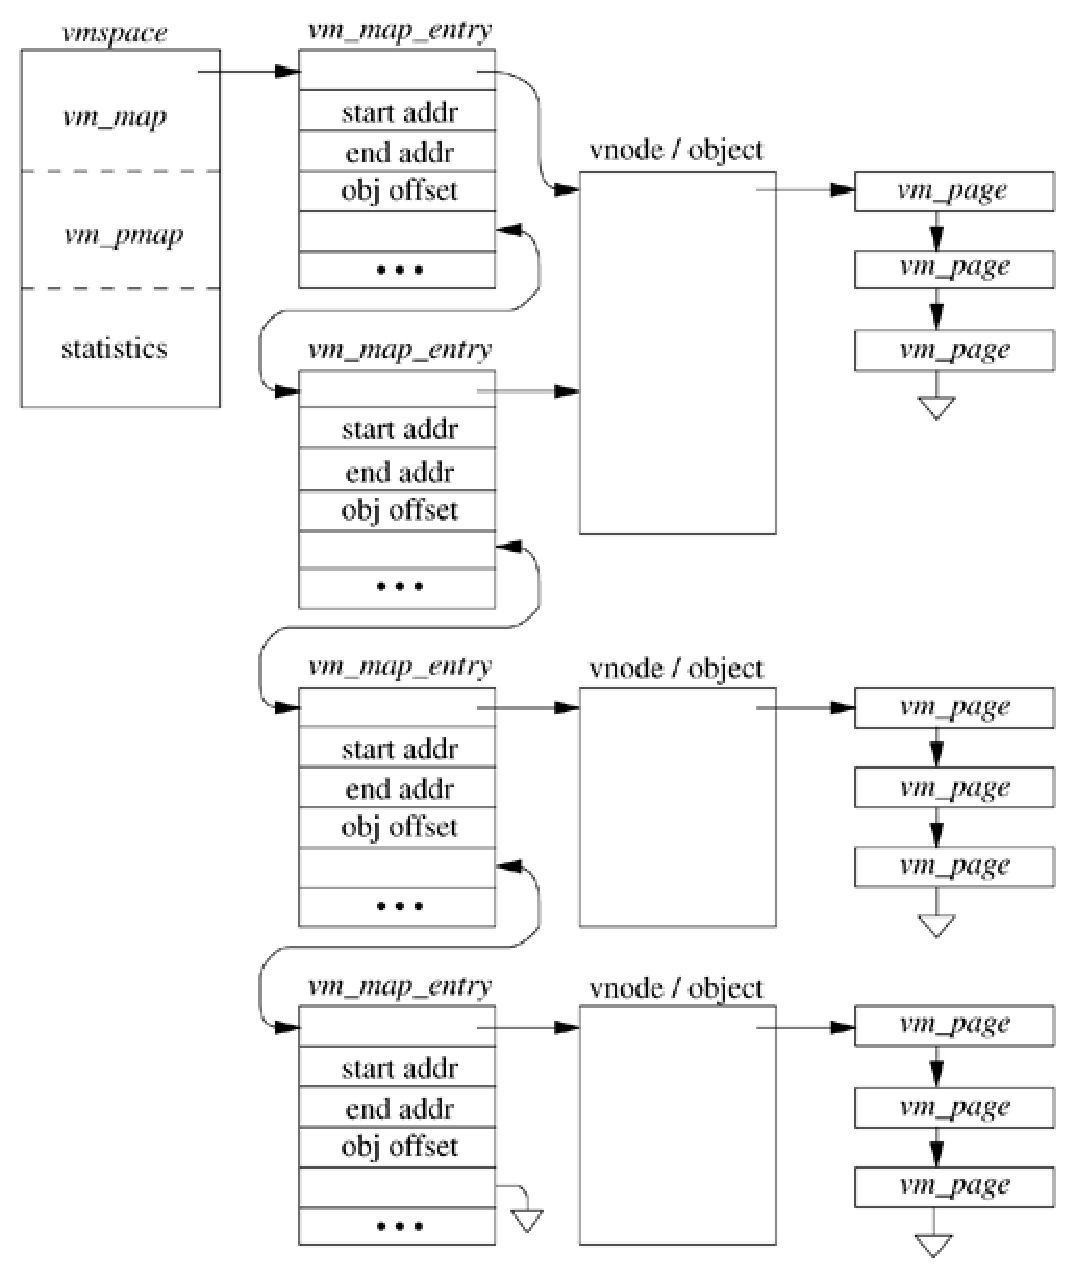
\includegraphics[width=.5\textwidth, height=.35\textheight]{freebsd.eps}
				\centering
				\caption{FreeBSD virtual memory schematic \cite{freeBSDMM}}
				\label{fig:mesh3}
			\end{figure}
	
			FreeBSD uses the schematic shown in figure 1 to implement virtual memory.
			The \textit{vmspace} structure has a \textit{vm\_map} structure which points to an ordered linked-list of \textit{vm\_map\_entry} nodes.
			Each \textit{vm\_map\_entry} node contains the starting and ending address of the process's contiguous region of virtual memory, as well as the offset from the starting address to the \textit{vm\_object}.
			Each \textit{vm\_object} that a \textit{vm\_map\_entry} points to has the same set of attributes, such as protection level.
			There are zero or more “shadow” \textit{vm\_objects} between a \textit{vm\_map\_entry} and its list of \textit{vm\_object}s.
			A shadow object records changes to the \textit{vm\_object}.
			When a change in memory is made, the shadow object stores a pointer to a new \textit{vm\_page} containing the changes and another pointer to the unmodified \textit{vm\_object}.
			A \textit{vm\_object} node contains a pointer to a linked-list of \textit{vm\_page}s.
			These pages makeup the physical memory cache of the \textit{vm\_object} \cite{freeBSDMM}. 
			
		\subsubsection{Page Management}
			FreeBSD places pages in one of five states \cite{freeBSDBook}.
			
			\textit{Wired:} Wired pages are locked in memory and can't be paged out.
			A page is in this state when it is in use by the kernel, the physical-memory pager, or a program specifies that the page should be locked via the \textit{mlock} call.
			
			\textit{Active:} Active pages are currently in use by one or more regions of virtual memory.
			
			\textit{Inactive:} Inactive pages are not currently in use and their data is out of date.
			Their data has not been updated to match the new writes in the backing store.
			
			\textit{Cache:} Cache pages contain data that is still in agreement with the backing store but are not currently in use.
			If an active page gets paged-out it will become a cached page.
			Pages in the cached list are similar to those in the \textit{inactive} list, except their contents are known.
	
			\textit{Free:} Free pages are no longer considered useful and will be overwritten.
			
			In summary, \textit{active} and \textit{wired} pages are those which are currently in use and can't be paged out to \textit{free}. 
			\textit{Inactive} pages are out of date and not in use, so they can be paged out.
			\textit{Cache} pages are those that are up to date and not in use.
			\textit{Cache} pages are kept around in case the system needs to page them in again soon.
			\textit{Free} pages are unused and will be overwritten.
	
	\subsection{Windows Implementation}
		\subsubsection{Memory Manager}	
			Windows has a \textit{memory manager} which handles all tasks related to allocating and managing memory. 
			The memory manager is responsible for fetching the physical memory mapped to by virtual memory, paging contents to disk when they become overcommitted, creating memory mapped files, managing copy-on-write memory, and managing large sparse address spaces \cite{windowsMM}.
			
			At a high level the memory manager handles all of the above in the same manner that Linux does.
			The use of page tables to access a virtual memory's corresponding physical memory is consistent with how Linux performs the translation.
			The \textit{page table} has a \textit{page table index}, \textit{page directory index}, and \textit{byte offset} that the memory manager uses to translate the virtual memory to physical memory.
	
		\subsubsection{Virtual Memory}
			\begin{figure}[H]
				\includegraphics[width=.6\textwidth, height=.35\textheight]{windowsMM.eps}
				\centering
				\caption{Windows virtual memory schematic \cite{windowsMM}}
				\label{fig:mesh4}
			\end{figure}
	
			Each process has a single \textit{page directory}, created by the memory manager, to map the location of all page tables for that process.
			The page directory is filled with \textit{page directory entries} (PDEs).
			PDEs contain data that describes the state and location of all the possible page tables for the process. 
	
			The memory management unit goes through the workflow below to translate the virtual address to a physical one \cite{windowsMM}.
			\begin{enumerate}
				\item{
					A privileged CPU register, CR3, is used to obtain the physical address of the page directory.
				}
				\item{
					The \textit{page directory index} located in the virtual address (as shown in figure 2) is used as an index into the page directory.}
				\item{
					The \textit{page table index} is used as an index into the page table to locate the PTE.}
				\item{
					If the PTE's \textit{valid bit} is clear, then a page fault occurs and the memory manager attempts to fetch the page.
					If the PTE's \textit{valid bit} is not clear, or the page shouldn't be accessed, then an access violation or bug check is generated}
				\item{
					The physical address is then fetched using the PFN field of the PTE to access the correct page frame.
					Then, the \textit{byte offset} is used to offset into the page frame to the requested physical address.}
			\end{enumerate}
		
		\subsection{Compare}
			Linux, FreeBSD, and Windows all translate virtual addresses to physical addresses at the granularity of a page.
			This means the smallest unit of protection at the hardware level is a page. 
			I believe this design decision was made because it simplifies virtual-to-physical translation by keeping a uniform memory size.
			
			The three operating systems' virtual-to-physical translation process is roughly the same as well.
			The location of needed indices and the page frame number are stored in different places, but the high level idea is the same.
			I believe all three operating systems use this process because it is efficient (having an index into a table allows for constant lookup) and systematic (easy to follow).



	
%************************FILESYSTEMS************************%
\section{File Systems}
	\subsection{Linux Implementation}
		In Linux, regular files are simply a stream of bytes.
		When an application requests to read a regular file, the stream of bytes are presented to the application along with an End Of File (EOF) condition.
		A regular file is referenced by the system by an inode.
		
		When a file is created, a unique number is associated to it.
		This is called the inode number.
		An inode holds information about the file such as \cite{llinuxInodeContents}:
		\begin{itemize}
			\item the file's permission mode
			\item the number of links in place for the file
			\item the file owners UID number
			\item the group GID number
			\item the file size represented in bytes
			\item the address of the datablocks
			\item the time the file was last modified
			\item the time any part of the inode was changed
		\end{itemize}
		
		When a file is not being used, its inode which resides on disk is called a disk inode.
		When the file is being used, the kernel places the inode onto a generic inode table and the inode now becomes a generic inode \cite{llinuxFiles}.
		
		In Linux, a directory is simply a file whose contents provide a mapping mechanism between the names of files in the directory and the file's actual datablocks.
		More specifically, a directory only holds the inode numbers and filenames of the files within it \cite{llinuxFiles}.

		\subsubsection{Ext4}
			For most Linux distributions the Ext file system is the default file system.
			Ext was created in 1992 and has since been revised three times leading to the Ext4, which was created in 2008.
			The Ext4 file system was designed to be backwards compatible. This means one can mount an Ext4 file system as Ext3.
			Ext4 includes newer features that reduce file fragmentation, allows for larger volumes and files, and uses delayed allocation to improve flash memory life.
			Ext4 is a journaling file system.
			This means before the operating makes a write to disk, metadata is written in a journal.
			This way if the power goes out in the middle of a disk write the operating system knows to finish the write from checking the journal.
			Without a journal the operating system isn't aware that it didn't finish a write, creating a possibility for corrupt data on disk. 
			When formatting an external drive that will be shared with other operating systems, one should not use Ext4 because Windows, macOS, and other devices can’t read Ext4 file systems \cite{llinuxEXT4}.

		\subsubsection{BtrFS}
			BtrFS, stands for “B-Tree File System.”
			BtrFS allows for drive pooling, on the fly snapshots, transparent compression, and online defragmentation \cite{llinuxEXT4}.

	\subsection{FreeBSD Implementation}
		\subsubsection{UFS}
			UFS stands for "Unix File System."
			UFS is split into two layers: an upper layer (called the UFS) and a lower layer (called the FFS).
			The upper layer contains the file system's directories in an inode structure and metadata such as permissions and ownership.
			The lower layer provides data containers implemented as inodes \cite{freebsdUFS}.
			
			In UFS2, the upper and lower layer are extended to add 64-bit block pointers.
			This allows for volumes to grow up to 8 zettabytes, variable-sized blocks, extended flag fields, and additional 'birthtime' stamps. 
			Since FreeBSD 7.0, UFS also supports filesystem journaling \cite{freebsdUFS}.
	
		\subsubsection{ZFS}
			ZFS supports a lot of advanced features including drive pooling, snapshots, and dynamic disk striping.
			Each file in ZFS has a checksum, so the file system can tell if a file is corrupted or not \cite{llinuxEXT4}.
			
			ZFS is more than just a file system. 
			ZFS combines the volume manager and the file system, which are traditionally kept separate.
			The file system is now aware of the underlying structure of the disks. 
			Traditional file systems could only be created on a single disk at a time. 
			If a user wants to use two disks, then they have to mount two separate file systems. 
			ZFS's combination of the volume manager and the file system solves this.
			This enhancement also allows multiple file systems to share a pool of available storage. 
			Due to ZFS's awareness of the physical layout, when an additional disk is added to the storage pool, each file system accessing that pool automatically grows \cite{freebsdZFS}.  


	\subsection{Windows Implementation}
		\subsubsection{FAT}
			The FAT file system is characterized by the file allocation table (FAT).
			Two copies of the file allocation table are kept on the system with one acting as a backup in case one becomes corrupted. 
			A disk utilizing the FAT file system is organized in clusters.
			The size of each cluster is determined by the size of the overall volume. 
			When a new file is created it is given the first open location on the drive, and an entry is added in to the FAT table.
			This entry in the FAT table either indicates that this is the file's last cluster or it points to the file's next cluster.
			A big disadvantage of the FAT file system is updating the FAT table is time consuming, and doing so is essential \cite{windowsFAT}.
	
		\subsubsection{NTFS}
			NTFS organizes files into sorted directories.
			Unlike the FAT file system, NTFS is independent of the underlying hardware of the system, such as 512 byte sectors. 
			NTFS is also independent of any special locations on the disk, such as FAT tables.
			According to Microsoft \cite{windowsFAT}, the goals of NTFS are to provide:
			\begin{itemize}
				\item{
					reliability, which is especially desirable for high end systems and file servers}
				\item{
					a platform for added functionality}
				\item{
					support POSIX requirements}
				\item{
					removal of the limitations of the FAT and HPFS file systems}
			\end{itemize}

	\subsection{Compare}
		Linux and FreeBSD are extremely similar in their underlying structure of directories and files.
		Because of this, most of the file systems supported by Linux are also supported by FreeBSD.
		Windows structures its file systems in a different manner.
		However, all three operating systems support the FAT file system.

\section{Conclusion}
	This document has explored processes and threads, devices, memory management, and file systems in the Linux, FreeBSD, and Windows operating systems.
	This document also stated differences, similarities, and opinions of why certain design and structural choices were made.

\bibliographystyle{IEEEtran}
\bibliography{references.bib}

\end{document}